\documentclass{beamer} 


% theme color
\definecolor{theme}{RGB}{28,90,127}
\definecolor{themelight}{RGB}{109,184,227}
\usecolortheme[named=theme]{structure} 

% outer color
%\usecolortheme{whale}
%\usecolortheme{seahorse}
\usecolortheme{dolphin}

% inner color
%\usecolortheme{lily}
\usecolortheme{orchid}
%\usecolortheme{rose}


% modified version of default frametitle with horizontal separation line
\makeatletter
\setbeamertemplate{frametitle}{
  \ifbeamercolorempty[bg]{frametitle}{}{\nointerlineskip}%
  \@tempdima=\textwidth%
  \advance\@tempdima by\beamer@leftmargin%
  \advance\@tempdima by\beamer@rightmargin%
  \begin{beamercolorbox}[sep=0.3cm,left,wd=\the\@tempdima]{frametitle}
    \usebeamerfont{frametitle}%
    \vbox{}\vskip-2ex%
    \if@tempswa\else\csname beamer@fteleft\endcsname\fi%
    \strut\insertframetitle\strut\par%
    {%
      \ifx\insertframesubtitle\@empty%
      \else%
      {\usebeamerfont{framesubtitle}\usebeamercolor[fg]{framesubtitle}\insertframesubtitle\strut\par}%
      \fi
    }%
    \vskip.45ex%
    \hrule %height .6pt%
    \vskip-1.45ex%
    \if@tempswa\else\vskip-.3cm\fi%
  \end{beamercolorbox}%
}
\makeatother

% clean up footer
\beamertemplatenavigationsymbolsempty
\setbeamertemplate{footline}[frame number]


% inner theme
\useinnertheme{rectangles}
\setbeamertemplate{itemize item}{\raise.30ex\hbox{\vrule width .80ex height .80ex}}
\setbeamertemplate{itemize subitem}{\raise.35ex\hbox{\vrule width .70ex height .70ex}}


\usepackage{appendixnumberbeamer,graphicx,amsmath,deriv,unit,short,booktabs,tikz,pgfplots,avg}
\graphicspath{{talkfig/}}
\usetikzlibrary{shapes}


\title{QGP parameter extraction via a global analysis of event-by-event flow coefficient distributions}

\author{Jonah Bernhard}

\institute{Preliminary exam}

\date{January 6, 2014}


\begin{document}



\section{Title}

\frame[plain,noframenumbering]{
  \begin{tikzpicture}[remember picture,overlay]
    \coordinate[xshift=.155\paperwidth] (middle) at (current page.center);
    \def\sep{.028\paperwidth}
    \def\extra{.8em}
    \node[align=right,anchor=east,xshift=-\sep] at (middle) {
      \color{theme}\large
      QGP parameter extraction via a global \\[\extra]
      \color{theme}\large
      analysis of event-by-event flow \\[\extra]
      \color{theme}\large
      coefficient distributions
    };
    \def\extra{.25ex}
    \node[align=left,anchor=west,xshift=\sep,yshift=-.42mm] at (middle) {
      \insertauthor \\[\extra]
      \scriptsize
      \insertinstitute \\[\extra]
      \scriptsize \insertdate
    };
    \def\lineheight{.66\paperheight}
    \draw[color=theme] (middle)++(0,-0.5*\lineheight) -- +(0,\lineheight);
  \end{tikzpicture}
}


\section{Background}


\begin{frame}{Model-to-data comparison}
  \vspace{.02\textwidth}
  \begin{tikzpicture}%[semithick]
    \node[draw,inner sep=.02\textwidth,text width=\textwidth,text centered] (data) {
      \textbf{Data} \\[2ex]
      \raisebox{.02\textwidth}{\includegraphics[width=.3\textwidth]{cmb}} %\\[1ex]
      \hspace{.01\textwidth}
      \includegraphics[width=.3\textwidth]{radar} %\\[1ex]
      \hspace{.01\textwidth}
      \raisebox{.005\textwidth}{\includegraphics[width=.3\textwidth]{atlasevent}}
    };
    \node[draw,inner sep=.02\textwidth,anchor=north west,text width=.3\textwidth,text centered,yshift=-.03\textwidth] (computer) at (data.south west) {
      \textbf{Computer model} \\[1ex]
      \includegraphics[width=\textwidth]{server}
    };
    \node[draw,inner sep=.02\textwidth,anchor=south east,text width=.3\textwidth,text centered,xshift=.6\textwidth] (end) at (computer.south east) {
      \textbf{Inferences} \\[1ex]
      \textbf{Predictions}
    };
    \draw[<->,thick] (computer) -| coordinate (x) (data);
    \draw[->,thick] (x) -| (end);
  \end{tikzpicture}
\end{frame}



\begin{frame}[label=mtd]{Model-to-data comparison:  heavy-ion collisions}
  \centering
  \def\tw{\textwidth}
  \vspace{.03\tw}
  \begin{tikzpicture}[semithick]
    \def\pw{.33\tw}
    %\matrix{\node{hello}; & \node{monkey}; \\ \node{hello}; & \includegraphics{evolution1} \\};
    %\matrix (m) [matrix of nodes,row sep=.03\tw,ampersand replacement=\&] {
    %  \includegraphics[width=\pw]{lhc} \&
    %  \node[draw,text width=.2\tw,text centered,inner sep=1em] {IC model, \\ $\tau_0$, $\eta/s$, \ldots}; \\
    %  %\node{\includegraphics[width=\pw]{atlasevent}}; \&
    %  %\node[text width=.60\tw,text centered] {
    %  %  \includegraphics[width=.20\tw]{evolution1}
    %  %  \includegraphics[width=.20\tw]{evolution2}
    %  %  \includegraphics[width=.20\tw]{evolution3} \\
    %  %  \includegraphics[width=.20\tw]{evolution4}
    %  %  \includegraphics[width=.20\tw]{evolution5}
    %  %}; \\
    %  %\node{\includegraphics[width=.5\tw]{atlas}}; \&
    %  %\node{\includegraphics[width=.3\tw]{flowdists}}; \\
    %};
    %%\path[->] (m-1-1) edge (m-2-1);
    \def\dx{.55\tw}
    \def\dy{.26\tw}
    \node (lhc) {\includegraphics[width=\pw]{lhc}};
    \node[below of=lhc,node distance=\dy] (atlasevent) {\includegraphics[width=\pw]{atlasevent}};
    \node[below of=atlasevent,node distance=\dy] (atlas) {\includegraphics[width=.5\tw]{atlas}};
    \node[right of=lhc,node distance=\dx,draw,text width=.28\tw,text centered,inner sep=2ex] (input) {\textbf{Model} \\ Initial conditions, \\ $\tau_0$, $\eta/s$, \ldots};
    \node[right of=atlasevent,node distance=\dx,text width=.60\tw,text centered] (evolution) {
      \includegraphics[width=.20\tw]{evolution1}
      \includegraphics[width=.20\tw]{evolution2}
      \includegraphics[width=.20\tw]{evolution3} \\
      \includegraphics[width=.20\tw]{evolution4}
      \includegraphics[width=.20\tw]{evolution5}
    };
    \node[right of=atlas,node distance=\dx] (flowdists) {\includegraphics[width=.3\tw]{flowdists}};
    \path[->] (lhc) edge (atlasevent) 
      (atlasevent) edge (atlas)
      (input) edge (evolution)
      (evolution) edge (flowdists);
    %\draw[->] (atlasevent) -- (atlas);
    %\draw[->] (input) -- (evolution);
    %\draw[->] (evolution) -- (flowdists);
    \draw[densely dashed,<->] (atlas) -- coordinate (m) (flowdists);
    \draw[densely dashed,->] (m) |- (input);
  \end{tikzpicture}
\end{frame}


\begin{frame}{Hot QCD matter}
  %\begin{tikzpicture}
  %  \draw[thick] (0,0) rectangle node {picture of RHIC} (200px,200px);
  %\end{tikzpicture}
  \begin{columns}
    \column{.5\textwidth}
    \begin{center}
      %\color{theme} \bf Normal matter
      Normal matter
      %\tikz\draw[thick] (0,0) rectangle node {hadrons \the\textwidth} (\textwidth,.618\textwidth);
      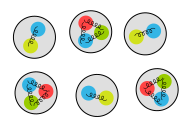
\includegraphics{confined}
    \end{center}
    \begin{itemize}
      \item Quarks and gluons confined to hadrons.
      \item Bound by strong nuclear force.
      \item Described by Quantum Chromodynamics (QCD).
    \end{itemize}

    \column{.5\textwidth}
    \begin{center}
      Quark-gluon plasma
      %\tikz\draw[thick] (0,0) rectangle node {QGP} (\textwidth,.618\textwidth);
      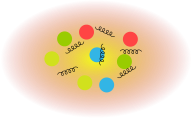
\includegraphics{deconfined}
    \end{center}
    \begin{itemize}
      \item QCD crossover transition $T~\sim~165$~MeV${}\sim 10^{12}$~K.
      \item Deconfined quarks and gluons.
      \item Hot and dense, short mean free path (fluid-like).
    \end{itemize}

  \end{columns}
\end{frame}


\begin{frame}{Relativistic heavy-ion collisions}
  \begin{itemize}
    \item Postulated that the universe was one large QGP in the first microseconds after the Big Bang.
    \item Small amounts created in relativistic heavy-ion collisions.
  \end{itemize}

  \bgs

  \begin{columns}
    \column{.5\textwidth}
    \centering
    \strut RHIC / BNL
    %\tikz\draw[thick] (0,0) rectangle node {aerial RHIC} (\textwidth,.618\textwidth);
    \includegraphics[width=\textwidth]{rhic} \\
    \strut Au+Au, Cu+Cu, U+U \\
    $\sqrt s \leq 200$ GeV

    \column{.5\textwidth}
    \centering
    \strut LHC / CERN
    %\tikz\draw[thick] (0,0) rectangle node {aerial LHC} (\textwidth,.618\textwidth);
    \includegraphics[width=\textwidth]{lhc} \\
    \strut Pb+Pb \\
    $\sqrt s = 2.76$ TeV
  \end{columns}
\end{frame}


\begin{frame}{Spacetime evolution}

  \centering

  \vspace{.06\textwidth}

  %\begin{columns}
  %  \column{.4\textwidth}
  %  \tikz\node[draw,thick,color=theme,minimum height=13mm]{\includegraphics[width=\textwidth]{evolution_alt}};
  %  \column{.6\textwidth}
  %  \tikz\node[draw,thick,color=theme,text width=\textwidth,minimum height=13mm,text badly centered]{Cannot directly resolve in time or space \\ 
  %    $\boldsymbol\rarr$ must use simulations to characterize};
  %\end{columns}

  %\small\hspace*{-2em}  \mbox{Cannot directly resolve in time or space $\rarr$ must use simulations to characterize} \\

  \begin{tikzpicture}
    \footnotesize
    \node (fig) {\includegraphics[width=.58\textwidth]{evolution_alt}};
    \draw[<->] (fig.north west) -- node[left] {$x \sim 10^{-14}$ m} (fig.south west) -- (fig.south east) node[right,yshift=.4ex] {$t \sim 10^{-23}$ s};
    %\draw[->] (fig.east) -- +(1em,0) node[right,anchor=west] {$t \sim 10^{-23}$ s};
    %\node[anchor=west] at (fig.east) {$\rarr t \sim 10^{-23}$ s};
  \end{tikzpicture}

  \vspace{.05\textwidth}

  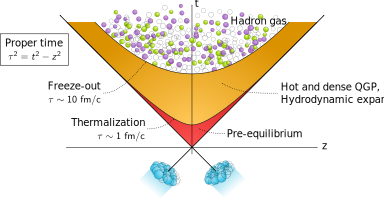
\includegraphics[width=\textwidth]{evolution_full}

  %\sms
  %\begin{description}
  %  \item[$t = 0$ fm/c] Nuclei collide (Lorentz-contracted discs).
  %  \item[$0\sim1$ fm/c] Pre-equilibrium / thermalization.
  %  \item[$1\sim10$ fm/c] Hot and dense QGP, hydrodynamic expansion.
  %  \item[{$\sim$}10 fm/c] Hadronic freeze-out.
  %  \item[${>}10$ fm/c] Hadron gas, particles stream into detector.
  %\end{description}
  %\mds

  %\tikz\node[draw,thick,color=theme,text width=.85\textwidth,text badly centered]{Cannot directly resolve in time or space \\ 
  %  $\boldsymbol\rarr$ must use computer models to characterize};

  %\begin{columns}[t]
  %  \column{.2\textwidth}
  %  \begin{center}
  %    \tikz\draw[thick] (0,0) rectangle node {discs} (\textwidth,\textwidth);
  %    $t = 0$ fm/c
  %  \end{center}
  %  \small
  %  Nuclei collide \\[1ex]
  %  Lorentz-contracted discs

  %  \column{.2\textwidth}
  %  \begin{center}
  %    \tikz\draw[thick] (0,0) rectangle node {pre-eq} (\textwidth,\textwidth);
  %    $0\sim1$ fm/c
  %  \end{center}
  %  \small
  %  Pre-equilibrium \\[1ex]
  %  Thermalization

  %  \column{.2\textwidth}
  %  \begin{center}
  %    \tikz\draw[thick] (0,0) rectangle node {hydro} (\textwidth,\textwidth);
  %    $1\sim10$ fm/c
  %  \end{center}
  %  \small
  %  Hot and dense QGP \\[1ex]
  %  Hydrodynamic expansion

  %  \column{.2\textwidth}
  %  \begin{center}
  %    \tikz\draw[thick] (0,0) rectangle node {freeze-out} (\textwidth,\textwidth);
  %    ${\sim}10$ fm/c
  %  \end{center}
  %  \small
  %  Hadronic freeze-out

  %  \column{.2\textwidth}
  %  \begin{center}
  %    \tikz\draw[thick] (0,0) rectangle node {gas} (\textwidth,\textwidth);
  %    ${>}10$ fm/c
  %  \end{center}
  %  \small
  %  Hadron gas \\[1ex]
  %  Particles stream into detector

  %\end{columns}

  %schematic evolution \\ described by viscous hydrodynamics
  %\begin{tabular}{ll}
  %  \toprule
  %  Approx.\ time (fm/c) & \\
  %  \midrule
  %  0 & nuclei collide (Lorentz-contracted discs) \\
  %  0--1 & pre-equilibrium / thermalization \\
  %  1--10 & hot and dense QGP, hydrodynamic expansion \\
  %  10 & hadronic freeze-out \\
  %  ${>}10$ & hadron gas \\
  %  \bottomrule
  %\end{tabular}
  %\begin{description}
  %  \item[$t = 0$ fm/c] nuclei collide (Lorentz-contracted discs)
  %  \item[0--1 fm/c] pre-equilibrium / thermalization
  %  \item[1--10 fm/c] hot and dense QGP, hydrodynamic expansion
  %  \item[{$\sim$}10 fm/c] hadronic freeze-out
  %  \item[$> 10$ fm/c] hadron gas
  %\end{description}

  %\begin{itemize}
  %  \item $t = 0$ fm/c:  
  %\end{itemize}
\end{frame}


%\begin{frame}{Boost invariance}
%  \begin{columns}
%    \column{.7\textwidth}
%    %\tikz\draw (0,0) rectangle node {\the\textwidth} (\textwidth,210pt);
%    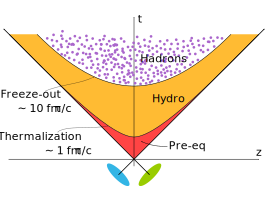
\includegraphics{boost}
%
%    \column{.3\textwidth}
%    \begin{flalign*}
%      \eta_s &= \frac{1}{2} \ln \frac{t + z}{t - z} & \\[1em]
%      \tau^2 &= t^2 - z^2
%    \end{flalign*}
%  \end{columns}
%  \centering
%  \mds
%  Approximate boost-invariance for $|\eta_s| \lesssim 3$.
%\end{frame}


%\begin{frame}{Spacetime evolution}
%  \vspace{.03\textwidth}
%  \tikz\draw (0,0) rectangle node {\the\textwidth} (\textwidth,220pt);
%\end{frame}


\begin{frame}{Collective behavior}
  \vspace{.5em}

  \centering
  \textbf{Strongly-interacting} fluids exhibit collective behavior \\

  \vspace{1.5em}

  \begin{columns}%[t]
    \column{.5\textwidth}
    %\tikz\draw[thick] (0,0) rectangle node {elliptic flow \the\textwidth} (\textwidth,.618\textwidth);
    %\color{red} $\partial_t v \propto \nabla P$
    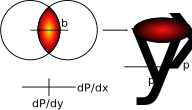
\includegraphics{ellipticflow} \\[1em]
    \footnotesize
    %\begin{tikzpicture}[scale=.8]
    %  \coordinate (L) at (0,0);
    %  \coordinate (R) at (1.3,0);

    %  \def\cl{(L) circle (1)}
    %  \def\cr{(R) circle (1)}

    %  \begin{scope}
    %    \clip\cl;
    %    \clip\cr;
    %    \shade[inner color=yellow,outer color=red] (.65,0) ellipse (.4 and .8);
    %  \end{scope}

    %  \draw[thick] \cl;
    %  \draw[thick] \cr;
    %  \draw[semithick,->] (L) -- (R) node[above] {$b$};

    %  \draw[semithick,<->] (-.4,-2) -- coordinate (a) ++(2.1,0) node[below] {$\partial P/\partial x$};
    %  \draw[semithick,<->] (a)++(0,.5) node[right] {$\partial P/\partial y$} -- ++(0,-1);

    %  \draw[very thick,->] (R)++(1.3,0) -- ++(.5,0) coordinate (b);

    %  \shade[inner color=red,outer color=black] (b)++(1.1,0) ellipse (.9 and .45);

    %\end{tikzpicture}

    Pressure gradient $\rarr$ fluid flow:
    \begin{equation*}
      (\epsilon + P) \pd{\vec v}{t} = -\vec\nabla P
    \end{equation*}
    %$(\epsilon + P) \partial_t\vec v \simeq -\nabla P$

    \column{.5\textwidth}
    %\tikz\draw[thick] (0,0) rectangle node {ultra-cold lithium} (\textwidth,\textwidth);
    %\includegraphics[height=.7\textheight]{lithium} %\\
    %\column{.18\textwidth}
    \includegraphics[width=\textwidth]{lithium} \\[1ex]
    \raggedleft \tiny K.~O'Hara, S.~Hemmer, M.~Gehm, S.~Granade, J.~Thomas, Science \textbf{298}, 2179 (2002).
  \end{columns}

  \vspace{1.5em}

  \hspace*{-1.5ex}\mbox{Initial-state spatial anisotropy $\implies$ Final-state momentum anisotropy}

  %\tikz[remember picture,overlay]\draw (current page.center)++(0,.2\paperheight) -- +(0,-.52\paperheight);
\end{frame}


\begin{frame}{Flow}

  %\begin{flushright}
  %  \tikz\draw[thick] (0,0) rectangle node {elliptic flow} (.4\textwidth,.2\textwidth);
  %\end{flushright}
  %\vspace{-10mm}
  %\begin{tikzpicture}[thick,->]
  %  \node (initial) {Initial-state spatial anisotropy};
  %  \node[below right of=initial,xshift=2.3cm] (final) {Converted to final-state momentum anisotropy};
  %  \node[below of=final] (flow) {Parameterized as collective flow $\color{theme}\boldsymbol{v_n}$};
  %  %\node[draw,above right of=initial,xshift=5cm,yshift=1cm,inner sep=1cm] {elliptic flow};
  %  \draw (initial.east) -| (final.north);
  %  \draw (final) -- (flow);
  %\end{tikzpicture}

  %\sms

  \begin{columns}
    \column{.5\textwidth}
    Momentum anisotropy parameterized by Fourier coefficients $\color{red} v_n$
    %\vspace{1em}
    \begin{equation*}
      \td N \phi \propto 1 + \sum_n {\color{red}v_n} \cos [ n(\phi - \psi_n) ]
    \end{equation*}
    \small
    $\phi$: Angle of transverse momentum \\
    $\psi_n$: Reaction-plane angle (phase)

    \column{.5\textwidth}
    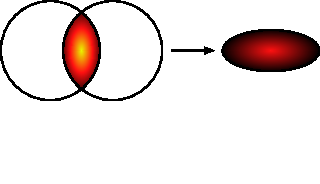
\includegraphics{ellipticflow_plain} \\[-1cm]
    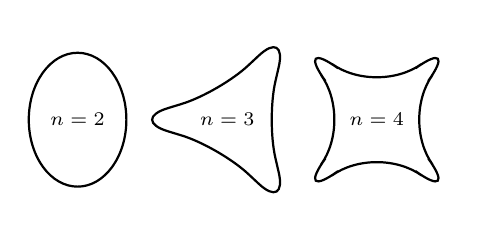
\begin{tikzpicture}[nodes={draw,thick}]
      \scriptsize
      \node[ellipse,minimum height=17mm] (2) {$n=2$};
      \node[right of=2,node distance=20mm,star, star points=3, rounded corners=5mm, minimum size=8mm, star point ratio=.3,rotate=30] (3) {};
      \node[draw=none,right of=2,node distance=19mm] {$n=3$};
      \node[right of=3,node distance=18mm,star, star points=4, rounded corners=7mm, minimum size=6mm, star point ratio=.2] {$n=4$};
    \end{tikzpicture}
  \end{columns}

  \vspace{3ex}

  \centering
  \tikz\node[draw,thick,color=theme,text width=.85\textwidth,text badly centered]{Flow provides essential evidence for the existence of a strongly-interacting QCD phase.};

\end{frame}


\begin{frame}{Event-by-event fluctuations}
  \begin{itemize}
    \item Average:  symmetric nuclei, almond-shape overlap.
      \begin{itemize}
        \item Large $v_2$, small $v_4,v_6,\ldots$, vanishing $v_3,v_5,\ldots$
      \end{itemize}
    \item Event-by-event:  randomly distributed nucleons, irregular overlap.
      \begin{itemize}
        \item All $v_n$ nonzero.
        \item Flow probability distributions $P(v_n)$.
      \end{itemize}
  \end{itemize}

  \mds

  %\centering
  \hspace*{-6mm}
  \begin{tabular}{ccc}
    Average peripheral & Fluctuating peripheral & Fluctuating central \\
    
\includegraphics[trim=0mm 4mm 0mm 4mm,clip]{averageperipheral} &
    \includegraphics[trim=0mm 4mm 0mm 4mm,clip]{toyglauber8} &
    \includegraphics[trim=0mm 4mm 0mm 4mm,clip]{toyglauber0}
  \end{tabular}
  %\includegraphics[width=.4\textwidth]{toyglauber}
  %\tikz\draw[thick] (0,0) rectangle node {compare average / toy glauber} (\textwidth,.35\textwidth);
\end{frame}


%\begin{frame}{Flow distributions}
%  \begin{itemize}
%    \item Measure $v_n$ event-by-event.
%    \item Construct flow probability distribution $P(v_n)$.
%    \item Possible with large particle multiplicity (LHC).
%    \item Probe QGP properties via mean, width, and shape of distributions.
%  \end{itemize}
%\end{frame}


\begin{frame}{Viscosity}
  \vspace{1em}

  \begin{columns}
    \column{.5\textwidth}
    \begin{itemize}
      \item Shear viscosity $\eta$ = fluid's resistance to shear flow.
      \item Strongly-interacting fluid \\ 
        $\color{theme}\boldsymbol\rarr$ short mean free path \\ 
        $\color{theme}\boldsymbol\rarr$ small $\eta$
      \item Viscosity damps collective behavior (flow).
    \end{itemize}

    \column{.5\textwidth}
    %\tikz\draw[thick] (0,0) rectangle node {shear viscosity (inkscape)} (\textwidth,.618\textwidth);
    %\begin{tikzpicture}
    %  \node (fig) {
\includegraphics{viscosity}};
    %  \node[align=left,anchor=west,xshift=-1ex] at (fig.east) {$\displaystyle \tau = \eta \pd{v_x}y$};
    %\end{tikzpicture}
    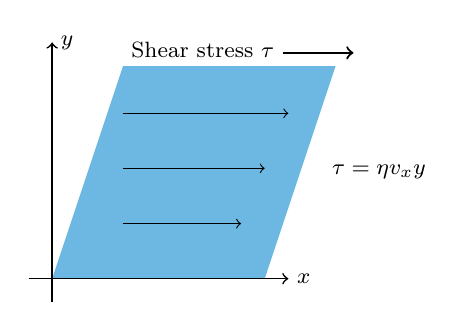
\begin{tikzpicture}[scale=.30]
      \footnotesize
      %\node (fig) {\includegraphics{viscosity}};
      %\node[align=left,anchor=west,xshift=-1ex] at (fig.east) {$\displaystyle \tau = \eta \pd{v_x}y$};
      %\node (o) at (0,0);
      \fill[color=themelight] (0,0) -- (3,9) coordinate (a) -- (12,9) -- coordinate (r) (9,0) -- cycle;
      \node[anchor=south west] (b) at (a.north west) {Shear stress $\tau$};
      \draw[semithick,->] (-1,0) -- (10,0) node[right] {$x$};
      \draw[semithick,->] (0,-1) -- (0,10) node[right] {$y$};
      \draw[thick,->] (b.east)++(0,-1ex) -- ++(3,0);
      \draw[->] (3,7.00) -- +(7,0);
      \draw[->] (3,4.67) -- +(6,0);
      \draw[->] (3,2.33) -- +(5,0);
      \node[align=left,anchor=west,xshift=1em] at (r.east) {$\displaystyle \tau = \eta \pd{v_x}y$};
    \end{tikzpicture}

    \mds

    %\begin{tikzpicture}
    %  \node (fig) {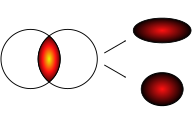
\includegraphics{ellipticflow_viscous}};
    %  \node[anchor=east,shift=({-.4ex,-2ex})] at (fig.north east) {small $\eta/s$};
    %  \node[anchor=east,shift=({-.3ex,1ex})] at (fig.south east) {large $\eta/s$};
    %\end{tikzpicture}
    %\tikz\draw[thick] (0,0) rectangle node {viscous $v_2$ (inkscape)} (\textwidth,.618\textwidth);
  \end{columns}

  \vspace{2em}

  \begin{equation*}
    \eta \sim nmv_\text{avg} \ell_\text{mf} \sim \epsilon \ell_\text{mf}/v_\text{avg} \sim \epsilon t_\text{mf}
  \end{equation*}
\end{frame}


\begin{frame}{QGP specific shear viscosity}
  \hspace{-1ex}\mbox{Specific shear viscosity = dimensionless ratio to entropy density, $\eta/s$.}
  \begin{equation*}
    \eta \sim \epsilon t_\text{mf}, \;
    s \sim n \quad \implies \quad
    \eta/s \sim (\epsilon/n) t_\text{mf} \gtrsim 1
  \end{equation*}
  Water $\eta/s \sim 300$ at STP, Helium $\eta/s \sim 2$ at 3 K, \\
  QGP $\eta/s \sim \mathcal O(10^{-1})$.
  
  \vspace{2em}

  \begin{columns}
    \column{.45\textwidth}
    \begin{tikzpicture}
      \footnotesize
      \node (fig) {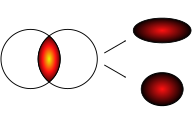
\includegraphics[width=\textwidth]{ellipticflow_viscous}};
      \node[anchor=north,xshift=2.5ex,text width=10ex,text centered] at (fig.north) {small $\eta/s$ \\ large $v_2$};
      \node[anchor=south,xshift=2.5ex,text width=10ex,text centered] at (fig.south) {large $\eta/s$ \\ small $v_2$};
    \end{tikzpicture}

    \column{.55\textwidth}
    Measuring QGP $\eta/s$:
    \begin{itemize}
      \item Observe experimental $v_n$.
      \item Run model with variable $\eta/s$.
      \item Constrain $\eta/s$ by matching $v_n$.
    \end{itemize}
  \end{columns}

\end{frame}


\begin{frame}{Simulations}
  \includegraphics[width=\textwidth]{evolution} \\[3ex]
  \begin{columns}
    \column{.2\textwidth}
    \column{.6\textwidth}
    Modern event-by-event model:
    \begin{itemize}
      \item Monte Carlo initial conditions
      \item (Pre-equilibrium)
      \item Viscous relativistic hydrodynamics
      \item Monte Carlo freeze-out
      \item Boltzmann transport
    \end{itemize}
    \column{.2\textwidth}
  \end{columns}
\end{frame}


\begin{frame}[label=ic]{Initial conditions}
  \begin{columns}
    \column{.6\textwidth}
    \begin{itemize}
      \item MC-Glauber model
        \begin{itemize}
          \item Randomly samples nucleon positions.
          \item Calculates energy density based on nucleon overlap.
        \end{itemize}
      \item \hyperlink{kln}{MC-KLN model}
        \begin{itemize}
          \item Randomly samples nucleon positions.
          \item Uses effective field theory to calculate gluon densities $\rarr$~proportional to energy density.
        \end{itemize}
      \item Many others.
    \end{itemize}
    %\color{red} timescale of nuclear fluctuations

    \column{.4\textwidth}
    %\tikz\draw[thick] (0,0) rectangle node {toy glauber} (\textwidth,.618\textwidth);
    %\tikz\draw[thick] (0,0) rectangle node {real glauber} (\textwidth,.618\textwidth);
    \centering
    \ \\
    Pb+Pb, $b = 8$ fm \\
    \includegraphics[trim=0mm 3mm 0mm 3mm,clip]{toyglauber8} \\
    \hspace{-7mm}\includegraphics{glb}
  \end{columns}
\end{frame}


\begin{frame}[label=hydro]{Viscous relativistic hydrodynamics}
  \bgs

  \begin{itemize}
    \item Ignore pre-equilibrium, expand medium without interactions.
    \item Start hydro evolution at time $\tau_0$ (must set explicitly).
    \item Conservation equations:
      \begin{equation*}
        \hyperlink{hydroeq}{
        \partial_\mu T^{\mu\nu} = 0, \quad
        T^{\mu\nu} = (\epsilon + P) u^\mu u^\nu - P g^{\mu\nu} + {\color{red}\pi^{\mu\nu}}.
        }
      \end{equation*}
    \item $\color{red}\pi^{\mu\nu}$ contains dissipative effects (viscosity).
    \item Equation of state $P = P(\epsilon)$.
  \end{itemize}

  \mds

  %\centering
  %\tikz\draw[thick] (0,0) rectangle node {comparison $\eta/s$ evolutions} (\textwidth,.35\textwidth);
  \footnotesize \hspace{3.2em} Initial condition \hspace{1.5em} Hydro $\eta/s = 0.04$ \hspace{1.3em} Hydro $\eta/s = 0.24$ \\
  \includegraphics{hydro}
\end{frame}


\begin{frame}{Hadronic freeze-out}
  \begin{columns}
    \column{.6\textwidth}
    \begin{itemize}
      \item Hydro stops at QCD transition, $T \sim 165$ MeV.
      \item Freezes into hadrons on hypersurface $\sigma$ according to Cooper-Frye formula
        \begin{equation*}
          E \frac{dN_i}{d^3p} = \int_\sigma f_i(x,p) \, p^\mu \, d^3\sigma_\mu
        \end{equation*}
      \item Randomly sample to produce an ensemble of particles.
    \end{itemize}

    \column{.4\textwidth}
    %\tikz\draw[thick] (0,0) rectangle node {freeze-out} (\textwidth,.618\textwidth);
    \centering
    \includegraphics[width=.6\textwidth]{evolution3} \\
    \includegraphics[width=.6\textwidth]{evolution4}
  \end{columns}


\end{frame}

\begin{frame}{Transport}
  \begin{columns}
    \column{.4\textwidth}
    %\tikz\draw[thick] (0,0) rectangle node {hadron gas} (\textwidth,.618\textwidth);
    \centering
    \includegraphics[width=.6\textwidth]{evolution4} \\
    \includegraphics[width=.6\textwidth]{evolution5}

    \column{.6\textwidth}
    \begin{itemize}
      \item Non-equilibrium Boltzmann transport
        \begin{equation*}
          \td{f_i(x,p)}{t} = \mathcal C_i(x,p)
        \end{equation*}
      \item Calculates final collisions and decays.
      \item Particles stream into ``detector''.
    \end{itemize}
  \end{columns}
\end{frame}




\section{Method}


%\begin{frame}{Model-to-data comparison}
%  %\centering
%  %\begin{tikzpicture}[node distance=2.3cm,semithick,scale=.9]
%  %  \node (input) [rectangle,draw,align=center] {\textbf{\color{theme} Input parameters} \\ $\eta/s$, $\tau_0$, $\alpha$, \ldots};
%  %  \node (model) [below of=input,rectangle,draw,align=center] {\textbf{\color{theme} Model} \\ initial conditions \\ viscous hydro \\ sampler \\ UrQMD};
%  %  \node (output) [below of=model,rectangle,draw,align=center] {\textbf{\color{theme} Output (observables)} \\ flow, multiplicity, \ldots};
%  %  \draw[->] (input) -- (model);
%  %  \draw[->] (model) -- (output);
%
%  %  \node (data) [right of=output,node distance=6.1cm,rectangle,draw,align=center] {
%  %    \textbf{\color{theme}Experimental data} \\[1ex]
%  %    %\vspace{2cm}\hspace{-.5cm}
%  %    \includegraphics[width=3cm]{atlas-phi}
%  %    \hspace{-.5cm}\vspace{-1cm}
%  %    \includegraphics[width=3cm]{atlas-flows} \\[1cm]
%  %    \includegraphics[width=3cm]{atlas-mult}
%  %  };
%
%  %  \draw[very thick,dashed,<->] (output) -- node[above] {\bf ?} (data); 
%  %\end{tikzpicture}
%  %\tikz\draw (0,0) rectangle node{\the\textwidth} (\textwidth,210pt);
%  \vspace{3mm}
%  \includegraphics[width=\textwidth]{mtd}
%\end{frame}



\againframe{mtd}


\begin{frame}{Computer experiments with slow models}
  \begin{columns}[t]
    \column{.5\textwidth}
    %\begin{center}
    %  \bf Challenges
    %\end{center}
    %\vspace{-2.2pt}
    %\hrule
    \begin{block}{\strut Challenges\vspace{-1pt}}
      \begin{itemize}
        \item Event-by-event models very computationally expensive, ${\sim}1$ hour per event.
        \item Need $\mathcal O(10^3)$ events per parameter-point to study fluctuations.
        \item Must vary all parameters simultaneously.
      \end{itemize}
    \end{block}

    \column{.5\textwidth}
    %\textbf{Solutions}
    %\begin{center}
    %  \bf Solutions
    %\end{center}
    %\hrule
    \begin{block}{\strut Strategies\vspace{-1pt}}
      \begin{itemize}
        \item Evaluate model at efficient pre-determined parameter points.
          \begin{itemize}
            \item Latin-hypercube sampling.
          \end{itemize}
        \item Interpolate between explicitly calculated points.
          \begin{itemize}
            \item Gaussian process emulator.
          \end{itemize}
      \end{itemize}
    \end{block}
  \end{columns}
\end{frame}


\begin{frame}{Latin-hypercube sampling}
  \begin{itemize}
    \item Random set of parameter points.
    \item Optimally fills parameter space.
    \item Avoids clusters.
  \end{itemize}

  \bgs 

  \centering
  %\tikz\draw[thick] (0,0) rectangle node {LHS samples} (\textwidth,.35\textwidth);
  \includegraphics{lhs}
  %\includegraphics<2>{lhs2}
\end{frame}


\begin{frame}[label=gp]{Gaussian processes}

  %A Gaussian \emph{process} is a generalization of a Gaussian \emph{distribution}:  \\
  %instead of drawing random numbers, draw random functions. {\color{red} formal definition} \\[1.5em]

  \begin{itemize}
    %\item A Gaussian process is a stochastic process where each point is normally distributed.
    \item \emph{A Gaussian process is a collection of random variables, any finite number of which have a joint Gaussian distribution.}
    \item Instead of drawing variables from a distribution, functions are drawn from a process.
  \end{itemize}



  \begin{columns}[c]
    \column{.55\textwidth}
    Require a covariance function, e.g.
    \begin{equation*}
      \text{cov}(x_1,x_2) \propto \exp \biggl[ -\frac{(x_1 - x_2)^2}{2\ell^2} \biggr]
    \end{equation*}
    Nearby points correlated, distant points independent.

    \column{.45\textwidth}
    \hyperlink{gengp}{\includegraphics[width=\textwidth]{gpr1}} \\[1ex]
    \raggedleft\tiny \emph{Gaussian Processes for Machine Learning}, \\ Rasmussen and Williams, 2006.
  \end{columns}

\end{frame}


\begin{frame}[label=emu]{Gaussian process emulators}
  \begin{itemize}
    \item Prior:  the model is a Gaussian process.
    \item Posterior:  Gaussian process conditioned on model outputs.
  \end{itemize}

  %\sms

  \hspace{-5mm}
  \begin{tikzpicture}
    \draw[thick,->] (0,0) node[left] (prior) {\includegraphics[width=.41\textwidth]{gpr1}} -- 
    node[above] {\hyperlink{training}{Training}} (1.8,0) node[right] (posterior) {\includegraphics[width=.41\textwidth]{gpr2}};
    \node[xshift=1.2ex] at (prior.north) {Prior};
    \node[xshift=1.5ex] at (posterior.north) {Posterior};
    %\node[align=right,anchor=east] at (posterior.south east) {\tiny Rasmussen and Williams, \emph{Gaussian processes for machine learning}.};
  \end{tikzpicture}
  
  %\sms

  \begin{itemize}
    \item Emulator is a fast surrogate to the actual model.
      \begin{itemize}
        \item More certain near calculated points.
        \item Less certain in gaps.
      \end{itemize}
  \end{itemize}
\end{frame}




\begin{frame}[label=atlas]{Experimental data}
  \begin{itemize}
    \item ATLAS event-by-event flow distributions $v_2,v_3,v_4$.
    \item Fit to \hyperlink{rice}{Rice / Bessel-Gaussian distribution}
      \begin{equation*}
        P(v_n) = \frac{v_n}{\delta_{v_n}^2} e^{ -\frac{(v_n)^2 + (v_n^\text{RP})^2}{2\delta_{v_n}^2} }
        I_0 \pfrac{v_n^\text{RP}v_n}{\delta_{v_n}^2}
      \end{equation*}
    \item Reduce to parameters $v_n^\text{RP}$, $\delta_{v_n}$.
  \end{itemize}
  
  %\vspace{-3ex}


  \centering
  \hyperlink{unfold}{\includegraphics[width=\textwidth]{atlas}}
  \flushright\vspace{-2ex} \tiny ATLAS Collaboration, JHEP {\bf 1311}, 183 (2013).
\end{frame}



\begin{frame}{Event-by-event model}
  Modern version of Duke+OSU model VISHNU \mbox{(Viscous Hydro and UrQMD)}:
  \begin{itemize}
    \item MC-Glauber \& MC-KLN initial conditions \\
      \hspace{1em} {\tiny H.-J.\ Drescher and Y.\ Nara, Phys.\ Rev.\ C {\bf 74}, 044905 (2006).}
    \item Viscous hydro \\
      \hspace{1em} {\tiny H.\ Song and U.\ Heinz, Phys.\ Rev.\ C {\bf 77}, 064901 (2008).}
    \item Cooper-Frye sampler \\
      \hspace{1em} {\tiny Z.\ Qiu and C.\ Shen, arXiv:1308.2182 [nucl-th].}
    \item UrQMD (Ultrarelativistic Quantum Molecular Dynamics) \\
      \hspace{1em} {\tiny S.\ Bass \emph{et.\ al.}, Prog.\ Part.\ Nucl.\ Phys.\  {\bf 41}, 255 (1998).} \\[-1ex]
      \hspace{1em} {\tiny M.\ Bleicher \emph{et.\ al.}, J.\ Phys.\ G {\bf 25}, 1859 (1999).}
  \end{itemize}

  \mds
  $\color{theme}\boldsymbol\rarr$ Tailored for running many events on Open Science Grid.
  
  %\vspace{.07\textheight}

  %\centering
  %\begin{tabular}{ll}
  %  \toprule
  %  Input parameters & Observables \\
  %  \midrule
  %  Normalization                           & \\
  %  WN/BC $\alpha$                          & $v_n$ distributions \\
  %  Thermalization time $\tau_0$            & Multiplicities \\
  %  Viscosity $\eta/s$                      & \ldots \\
  %  Shear relaxation time $\tau_\Pi$ & \\
  %  \bottomrule
  %\end{tabular}

\end{frame}





\begin{frame}{Computer experiment design}
  \begin{itemize}
    \item Six centrality bins 0--5\%, 10--15\%, \ldots\ 50--55\%.
    \item 256 Latin-hypercube points, five input parameters:
      \begin{itemize}
        \item Normalization
        \item IC-specific parameter
        \item Thermalization time $\tau_0$
        \item Viscosity $\eta/s$
        \item Shear relaxation time $\tau_\Pi$
      \end{itemize}
  \end{itemize}
  \begin{itemize}
    \item Massive parallelization on Open Science Grid.
    \item Completed 1000--2000 events per centrality bin and input-parameter point.
      \begin{itemize}
        \item 3.5 million total
        \item 0.5 $\mu\text{b}^{-1}$  (ATLAS:  7 $\mu\text{b}^{-1}$)
      \end{itemize}
  \end{itemize}

  %\bgs
  %\begin{itemize}
  %  \item (6 centrality bins) $\times$ (3 flow coefficients) = 18 flow ``categories''
  %  \item $v_2$ 0--5\% and $v_2$ 40--45\% are representative.
  %\end{itemize}
\end{frame}


\begin{frame}{Open Science Grid usage}
  \begin{tikzpicture}
    \node (fig) {\includegraphics[width=\textwidth]{osghours}};
    \node[anchor=south,yshift=-1ex,xshift=1.7ex] at (fig.north) {CPU hours per day};
    \node[anchor=south west,yshift=-1ex,xshift=1ex] at (fig.north west) {\small 250,000};
    \node[anchor=south west,yshift=1.8cm,xshift=.8cm] at (fig) {red = Me};
  \end{tikzpicture}
  \centering
  Completed KLN design (1.5 million events) in two weeks.
\end{frame}


\section{Results}


\begin{frame}{Model flow distributions}
  \vspace{6mm}
  \hspace{-3mm}
  \includegraphics{allcurves}
  %\the\textheight
  %\tikz\draw (0,0) rectangle (\textwidth,.8\textheight);
\end{frame}



\begin{frame}[label=scatter]{Input-output summary}
  \vspace{6mm}
  \hspace{-3mm}
  \hyperlink{linear}{
    \includegraphics<1>{scatters-glb}
    \includegraphics<2>{scatters-kln}
  }
\end{frame}




\begin{frame}{Best parameter points}
  \begin{columns}
    \column{.6\textwidth}
    \vspace{3mm}

    \scriptsize\raggedleft Best Latin-hypercube points by average $v_n$\ \ \ \\[.5ex]
    \includegraphics{bestavg}

    \column{.4\textwidth}
    %\begin{tabular}{lllll}
    %  \toprule
    %  & $\alpha\mid\lambda$ & $\tau_0$ & $\eta/s$
    %  \midrule
    %  \bottomrule
    %\end{tabular}
    %\begin{equation*}
    %  \alpha = 0.27,\;
    %  \tau_0 = 0.46 \ut{fm/c},\;
    %  \eta/s = 0.026,\;
    %  \tau_\Pi = 1.0 \ut{fm/c};
    %\end{equation*}
    %\begin{equation*}
    %  \lambda = 0.25,\;
    %  \tau_0 = 0.70 \ut{fm/c},\;
    %  \eta/s = 0.21,\;
    %  \tau_\Pi = 0.28 \ut{fm/c}.
    %\end{equation*}
    \small
    OSU results, same model \\[1em]
    dashed: Glauber $\eta/s = 0.08$ \\
    solid: KLN $\eta/s = 0.20$ \\[1ex]
    \begin{tikzpicture}
      \small
      \node (fig) {\includegraphics[width=\textwidth]{osu}};
      \node[anchor=east,shift=({-1.2em,3.2em})] at (fig.east) {$v_2$};
      \node[anchor=east,shift=({-1.2em,-1.3em})] at (fig.east) {$v_3$};
    \end{tikzpicture} \\
    %\includegraphics[width=\textwidth]{osu} \\
    \raggedleft\tiny Z. Qiu, C. Shen, and U.~Heinz, \\ Phys.\ Lett.\ B {\bf 707}, 151 (2012).
  \end{columns}
\end{frame}



\begin{frame}{Constraining $\eta/s$}
  \vspace{3mm}
  \small
  Points:  average $\eta/s$ of best 10 Latin-hypercube points by average $v_n$ \\
  Error bars:  standard deviation of best 10 \\
  Dashed lines:  canonical $\eta/s$ (Glauber 0.08, KLN 0.20) \\[1em]
  \includegraphics{preferredeta}
\end{frame}


\section{Conclusion}

\begin{frame}[label=conc]{Summary \& outlook}
  \begin{itemize}
    \item Framework for massive event-by-event model-to-data comparison:  new level of knowledge-extraction capability.
    \item Preliminary results consistent with previous work.
      \bgs
    \item Improve goodness of fit:  \hyperlink{likelihood}{beyond average flow}.
    \item Emulator:  vary single parameters independently, determine best-fit parameter values.
    \item Calibrate simultaneously on other observables, e.g.\ multiplicity.
    \item Repeat with more advanced models, especially initial conditions.
  \end{itemize}
\end{frame}



\appendix

\def\backbutton#1{
  \tikz[remember picture,overlay]\node[anchor=south west] at (current page.south west) {\hyperlink{#1}{\footnotesize\color{theme}$\blacktriangleleft$}};
}

\begin{frame}[plain,noframenumbering]{}
  \centering
  \Large
  backup slides
\end{frame}


\begin{frame}[label=kln]{Color glass condensate}
  \begin{columns}
    \column{.5\textwidth}
    \begin{itemize}
      \item High energy / small $x$:  parton distribution functions dominated by gluons.
      \item Gluons overlap coherently \\ $\rarr$ condensate state.
    \end{itemize}

    
    \column{.5\textwidth}
    \includegraphics[width=\textwidth]{saturation}

    \begin{equation*}
      x = p_T e^{\pm y}/\sqrt s
    \end{equation*}
  \end{columns}

  \backbutton{ic}
\end{frame}


\begin{frame}[label=hydroeq]{Viscous hydro}
  \small\vspace{2em}

  Conservation of energy and momentum:
  \begin{equation*}
    \partial_\mu T^{\mu\nu} = 0
  \end{equation*}
  Stress-energy tensor:
  \begin{equation*}
    T^{\mu\nu} = T^{\mu\nu}_\text{ideal} + \pi^{\mu\nu}
  \end{equation*}
  Ideal part: 
  \begin{equation*}
    T^{\mu\nu}_\text{ideal} = (\epsilon + P) u^\mu u^\nu - P g^{\mu\nu}
  \end{equation*}
  Shear viscosity correction:
  \begin{equation*}
    \pi^{\mu\nu} = \eta \nabla^{\langle\mu}u^{\nu\rangle}
  \end{equation*}
  Symmetric and traceless:
  \begin{equation*}
    \nabla^{\langle\mu}u^{\nu\rangle} = \nabla^\mu u^\nu + \nabla^\nu u^\mu - \tfrac{2}{3} \Delta^{\mu\nu} \nabla_\alpha u^\alpha
  \end{equation*}
  Projection orthogonal to four velocity:
  \begin{equation*}
    \Delta^{\mu\nu} = g^{\mu\nu} - u^\mu u^\nu \qquad
    \nabla_\mu = \Delta^\alpha_\mu \partial_\alpha
  \end{equation*}
  %\begin{align*}
  %  \partial_\mu T^{\mu\nu} &= 0 \\
  %  T^{\mu\nu} &= T^{\mu\nu}_\text{ideal} + \pi^{\mu\nu} & \quad\text{stress-energy tensor} \\
  %  T^{\mu\nu}_\text{ideal} &= (\epsilon + P) u^\mu u^\nu - P g^{\mu\nu} & \quad\text{ideal part} \\
  %  \pi^{\mu\nu} &= \eta \nabla^{\langle\mu}u^{\nu\rangle} & \\
  %  \Delta^{\mu\nu} &= g^{\mu\nu} - u^\mu u^\nu & \\
  %  \nabla_\mu &= \Delta^\alpha_\mu \partial_\alpha &
  %\end{align*}

  \backbutton{hydro}
\end{frame}


%\begin{frame}[label=lqcd]{Lattice QCD}
%
%\end{frame}


%\begin{frame}[label=boltz]{Boltzmann transport}
%
%\end{frame}


\begin{frame}[label=gengp]{Generating Gaussian processes}
  \begin{columns}
    \column{.67\textwidth}
    \begin{itemize}
      \item Choose a set of input points $X_*$.
      \item Choose a covariance function, e.g.\
        \begin{equation*}
          k(x_i,x_j) = \exp[-(x_i-x_j)^2/2]
        \end{equation*}
        and create covariance matrix $K(X_*,X_*)$.
      \item Generate MVN samples (GPs)
        \begin{equation*}
          \vec f_* \sim \mathcal N[\vec 0,K(X_*,X_*)].
        \end{equation*}
    \end{itemize}

    \column{.33\textwidth}
    \includegraphics[width=\textwidth]{gpr1}
  \end{columns}

  \backbutton{gp}
\end{frame}


\begin{frame}[label=training]{Training the emulator}
  \begin{itemize}
    \item Make observations $\vec f$ at training points $X$.
    \item Generate conditioned GPs
        \begin{align*}
          \vec f_* | X_*,X,\vec f &\sim \mathcal N[K(X_*,X)K(X,X)^{-1}\vec f, \\
          &\qquad {} K(X_*,X_*) - K(X_*,X)K(X,X)^{-1}K(X,X_*)].
        \end{align*}
  \end{itemize}

  \centering

  \begin{tikzpicture}
    \draw[thick,->] (0,0) node[left] (prior) {\includegraphics[width=.35\textwidth]{gpr1}} -- (1,0) node[right] (posterior) {\includegraphics[width=.35\textwidth]{gpr2}};
    \node[xshift=1.2ex] at (prior.north) {Prior};
    \node[xshift=1.5ex] at (posterior.north) {Posterior};
  \end{tikzpicture}

  \backbutton{emu}
\end{frame}


\begin{frame}[label=rice]{Rice / Bessel-Gaussian distribution}
  \vspace{1em}

  \begin{itemize}
    \item Flow vectors follow bivariate Gaussian
      \begin{equation*}
        P(\vec v_n) = \frac{1}{2\pi\delta_{v_n}^2} e^{ -\frac{(\vec v_n - \vec v_n^\text{RP})^2}{2\delta_{v_n}^2} }.
      \end{equation*}
    \item Integrate out angle
      \begin{equation*}
        P(v_n) = \frac{v_n}{\delta_{v_n}^2} e^{ -\frac{(v_n)^2 + (v_n^\text{RP})^2}{2\delta_{v_n}^2} }
          I_0 \pfrac{v_n^\text{RP}v_n}{\delta_{v_n}^2}.
      \end{equation*}
  \end{itemize}

  \vspace{1em}

  \centering
  \includegraphics[width=.7\textwidth]{rice}
  
  \backbutton{atlas}
\end{frame}


\begin{frame}[label=unfold]{Finite multiplicity and unfolding}
  \def\obs{^\text{obs}}

  \begin{itemize}
    \item Observed flow smeared by finite multiplicity and nonflow
      \begin{equation*}
        P(v_n\obs) = \int P(v_n\obs|v_n) P(v_n) \, dv_n
      \end{equation*}
      where $P(v_n\obs|v_n)$ is the response function.
    \item Pure statistical smearing $\rarr$ Gaussian response
      \begin{equation*}
        P(v_n^\text{obs}|v_n) = \frac{v_n^\text{obs}}{\delta_{v_n}^2} e^{ -\frac{(v_n^\text{obs})^2 + (v_n)^2}{2\delta_{v_n}^2} }
          I_0 \pfrac{v_nv_n^\text{obs}}{\delta_{v_n}^2}.
      \end{equation*}
    \item $v_n^\text{RP}$ unaffected; width increased as
      \begin{equation*}
        \delta_{v_n}^2 \rarr \delta_{v_n}^2 + 1/2M.
      \end{equation*}
  \end{itemize}

  \backbutton{atlas}
\end{frame}



\begin{frame}[label=likelihood]{Likelihood}
  \vspace{1em}

  Given experimental observations $y_i$ with errors $\sigma_i$ and model predictions $\theta_i$, what is the likelihood that the model
  describes reality?
  \begin{equation*}
    \mathcal L \sim \exp \biggl[ -\sum_i \frac{(y_i-\theta_i)^2}{2\sigma_i^2} \biggr] 
  \end{equation*}
  Or as a null hypothesis:  can the model be rejected based on comparison to the data?  (e.g.\ If a coin is flipped $N$ times and yields
  heads each time, what is the probability that it is fair?)

  \vspace{1em}

  \centering
  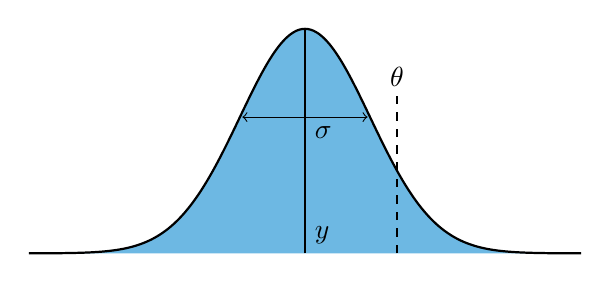
\begin{tikzpicture}
    \begin{axis}[domain=-3:3,hide axis,height=5cm,width=10cm]
      \addplot[mark=none,samples=100,fill=themelight,smooth,thick] {exp(-x*x)};
      \draw (axis cs:0,0) node[above right] {$y$} -- (axis cs:0,1);
      \draw[<->] (axis cs:-.68,.607) -- node[below right] {$\sigma$} (axis cs:.68,.607);
      \draw[semithick,dashed] (axis cs:1,0) -- (axis cs:1,.7) node[above] {$\theta$};
    \end{axis}
  \end{tikzpicture}

  \backbutton{conc}
\end{frame}




\begin{frame}[label=linear]{Linear fit example}
  \vspace{3mm}
  \includegraphics{linear}

  \backbutton{scatter}
\end{frame}






\end{document}
